\chapter{Modello teorico di Controllo}\label{cap:controlModel}

\begin{minipage}{12cm}\textit{Se lo si desidera, utilizzare questo spazio per inserire un breve riassunto di ci\`o che verr\`a detto in questo capitolo. Inserire solo i punti salienti.}
\end{minipage}

\vspace*{1cm}

\section{Obiettivo di controllo}
Come accennato nella sezione "\nameref{sub:parametriMisurati}" (\ref{sub:parametriMisurati}), attraverso il controllo e attuazione della corrente nel Primario del trasformatore, si punta controllare la corrente presente sul primario del trasformatore, e sempre come detto nella sezione \ref{sub:parametriMisurati}, non essendo possibile misurare la corrente di plasma direttamente, si usa la sua misura indiretta che passa per la $ F_{em} $.\\
In questa tesi l'obiettivo che ci si è ripromessi di raggiungere è la creazione di un controllo ad errore nullo sulla corrente di plasma.\vspace{-4mm}
\begin{figure}[h]
	\centering
	\caption[Sistema da controllare a blocchi con $ P(s) $]{Sistema da controllare a blocchi con $ P(s) $}
	\vspace{1mm}
	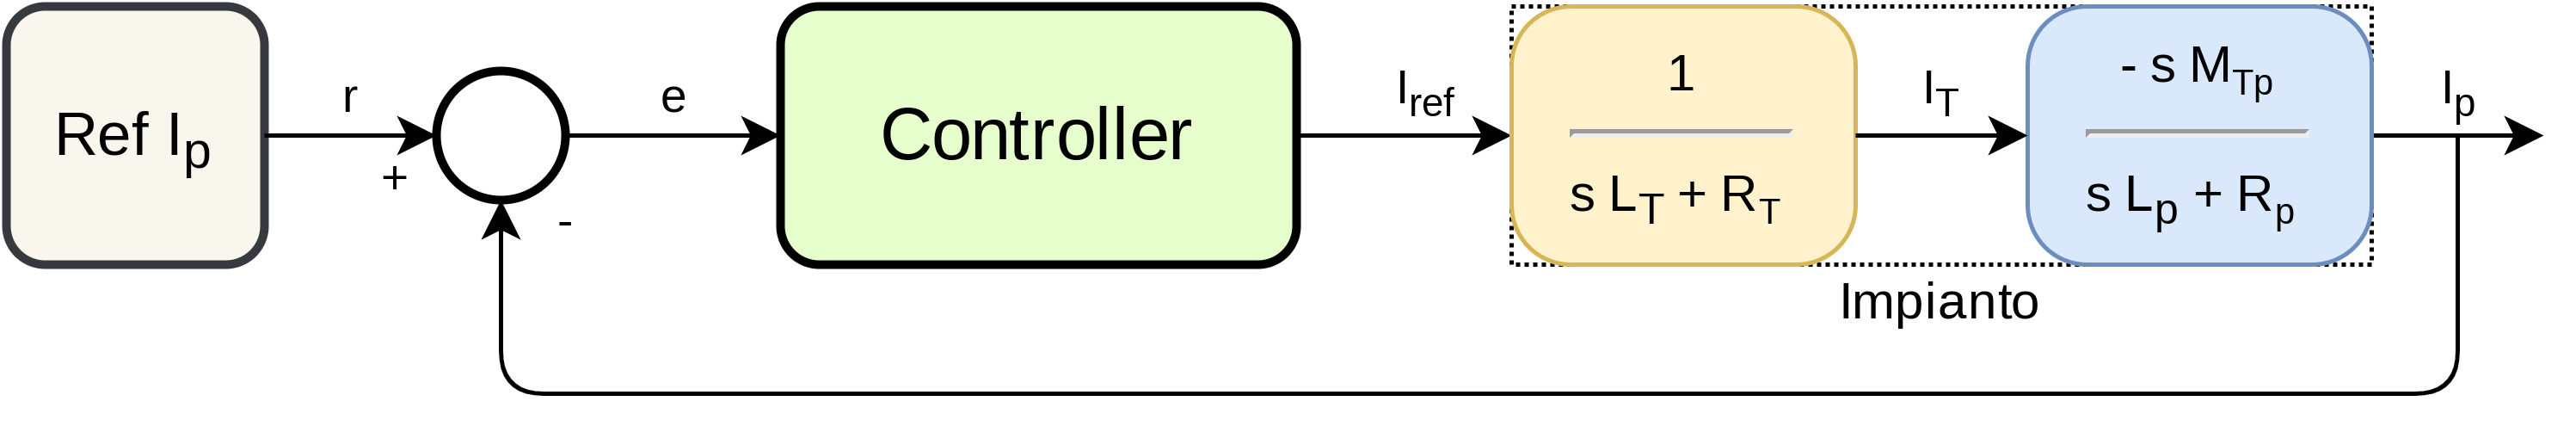
\includegraphics[width=1\textwidth]{ModelloMatematico/SchemiBlocchi.png}
\end{figure}\vspace{-4mm}

\noindent
Come visto però nella sezione, "\nameref{sub:parametriMisurati}", la misura a nostra disposizione il voltmetro la $V_2$, che equivale alla  diagnostica di $ V_{loop} $ in un impianto reale.\\
Dall'equazione della dinamica del plasma \ref{eq:correntePlasmaDinamica} siamo in grado di ricavare che:
\begin{empheq}[box=\mathStep]{equation*}
	V_2 = I_p \cdot R_p = F_{em} - L_p \cdot \dot{I_p}
\end{empheq}

\noindent
La quale, trascurando la dinamica del filtro RC di misura (che comunque è $ >= f_{tic} $ di acquisizione e di conseguenza ha una dinamica estremamente più rapida del segnale da misurare)  permette di ricavare, invertendo il segno della tensione come della corrente per avere i segni positivi, la funzione di ingresso-uscita dalla $ I_{ref} $ alla $ V_2 $ pari a:
\begin{empheq}[box=\mathCalc]{equation}
	V_2(s) = I_p(s) \cdot- R_p \Rightarrow V_2(s) = P_{pos}(s) \cdot I_{ref}(s) \cdot R_p
\end{empheq}
Da cui la funzione di trasferimento complessiva diventa:
\begin{empheq}[box=\mathCalc]{equation}\label{eq:FunxTrasImpiantoIrefV2}
	\frac{V_2(s)}{I_{ref}(s)} = P_{pos}(s) \cdot R_p
\end{empheq}
E il riferimento di corrente di plasma, diventa un riferimento di tensione secondo l'equazione di conversione:
\begin{empheq}[box=\mathCalc]{equation}\label{eq:V2RefEquivalent}
	V_{2_{ref}} = I_{p_{ref}} \cdot R_p
\end{empheq}

\begin{figure}[h]
	\centering
	\caption[Sistema da controllare ingresso-uscita reale]{Sistema da controllare ingresso-uscita reale}
	\vspace{1mm}
	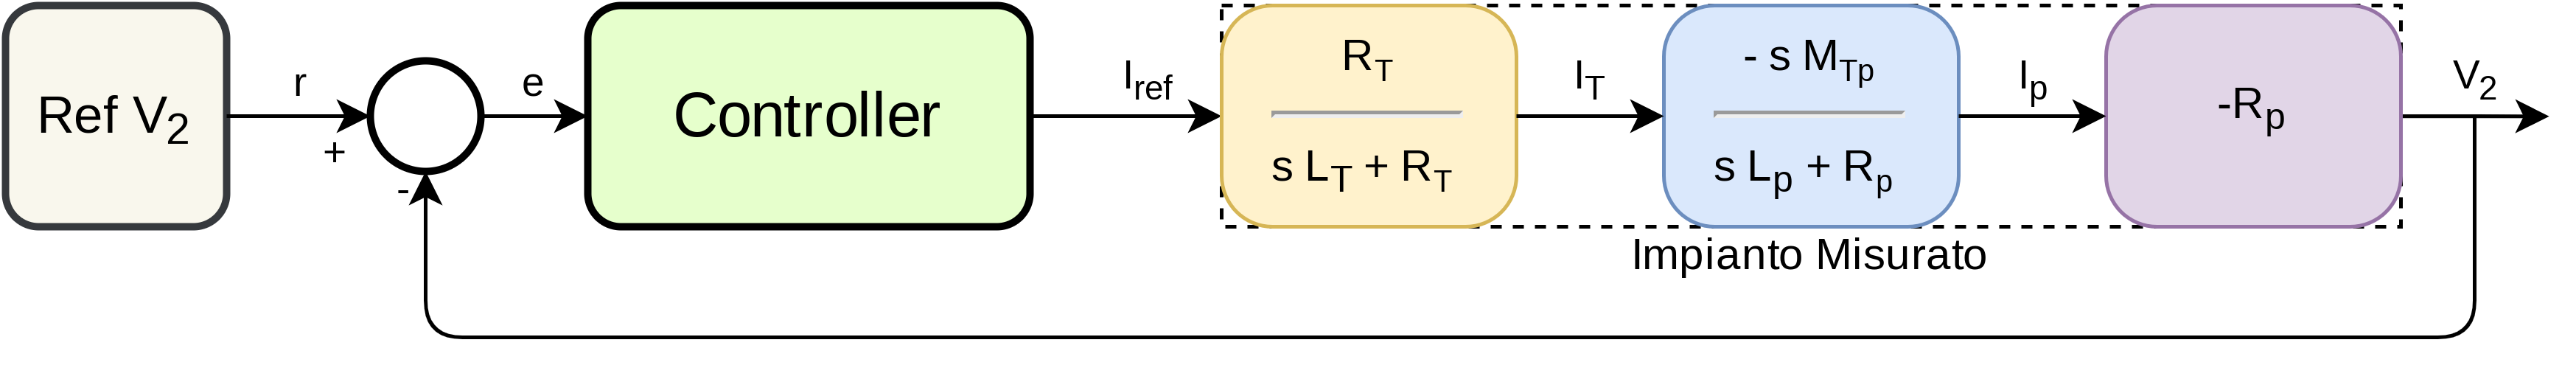
\includegraphics[width=1\textwidth]{ModelloMatematico/SchemiBlocchi-SchemaBlocchiV2Out.png}
\end{figure}

\newpage
\section{Teorema del valore iniziale e del valore finale}
Prima di procedere con il calcolo del controllore per i nostri scopi, è bene ricordare il \nameref{th:valIniziale} e il \nameref{th:valFinale} della Trasformata di Laplace (\cite*{Laplace}):

\begin{teorema}[Teorema del valore iniziale \label{th:valIniziale}]
	Se una funzione reale $ f  $ ha trasformata razionale $ F(s) $ con grado del denominatore maggiore del grado del numeratore (vale comunque sotto ipotesi ancora più larghe , purché $ F $ sia non razionale e $ f(0^+) $ esista) allora:
	\begin{empheq}[box=\mathResult]{equation} \label{eq:valIniziale}
		f(0^+) = \lim\limits_{s \rightarrowtail \inf} s \cdot F(s)
	\end{empheq}
\end{teorema}

\begin{teorema}[Teorema del valore finale \label{th:valFinale}]
	Se una funzione reale $ f  $ ha trasformata razionale $ F(s) $ con grado del denominatore maggiore del grado del numeratore e \underline{radici del denominatore (\textbf{poli}) nell’origine e o a parte reale negativa},\\
	allora:
	\begin{empheq}[box=\mathResult]{equation} \label{eq:valIniziale}
		\lim\limits_{t \rightarrowtail \inf} f(t) = \lim\limits_{s \rightarrowtail 0} s \cdot F(s)
	\end{empheq}
\end{teorema}

Questi 2 Teoremi chiave, permettono di risolvere comodamente le equazioni differenziali, e quindi calcolare in maniera semplice il controllore che permette di ottenere gli obiettivi di controllo che ci si è prefissati di ottenere.

\newpage

\section{Controllo a errore nullo}
Definiamo ora $ P_m(s) $ come l'impianto Reale misurato tra la corrente di riferimento $ I_{ref} $ del primario, e la tensione del campo elettrico $ V_2 $ sul secondario.\\
Ne segue che la funzione di trasferimento complessiva è pari a:
\begin{empheq}[box=\mathCalc]{equation}\label{eq:impiantoMisurato}
	P_m(s)= \frac{V_2(s)}{I_{ref}(s)} = \frac{s M_{Tp} \cdot R_p}{( s L_p + R_p)(s L_T + R_T)} = \frac{s M_{Tp} \cdot R_p}{s^ 2L_p L_T + s(L_p R_T + L_T R_p) + R_p R_T}
\end{empheq}
Essendo il nostro obiettivo quello di portare $ e \rightarrowtail 0$ per $ t\rightarrowtail \inf $ con riferimenti $ r = cost $, ci calcoliamo la funzione sensitività $ W_{er}(s) $ (\textit{sensitivity transfer function}) e con il \nameref{th:valFinale} progetteremo il controllore $ C(s) $ che realizza l'obiettivo:\\
\begin{vwcol}[widths={0.5,0.5}, sep=8mm, rule=0px]
	\vspace{-12mm}
	\begin{empheq}[box=\mathStep]{equation*}
		W_{er}(s) = \frac{e(s)}{r(s)} = \frac{1}{1 + P_m(s)C(s)}
	\end{empheq}
	\newpage
	{\color{red}(Sensitivity transfer function)}
\end{vwcol}
\vspace{5mm}
\begin{vwcol}[widths={0.5,0.5}, sep=8mm, rule=0px]
	\vspace{-8mm}
	\begin{empheq}[box=\mathStep]{equation*}
		r(t) = cost \rightarrow r(s)= \frac{K_r}{s}
	\end{empheq}
	\newpage
	Trasformata di Laplace del riferimento
\end{vwcol}

Da cui, applicando il \nameref{th:valFinale} otteniamo:
\begin{empheq}[box=\mathCalc]{equation}\label{eq:dinamicaErroreRifCost}
	\lim\limits_{t \rightarrowtail \inf} e(t) = \lim\limits_{s \rightarrowtail 0} s \cdot W_{er}(s) \cdot r(s) = s \cdot \frac{K_r}{1 + P_m(s)C(s)}
\end{empheq}
% Riscrivere C e P in forma generale mettendo in evidenza den, num, K e s^rho, poi fare i calcoli e mostrare i risultati.
Svolgendo i calcoli abbiamo che:
\begin{center}
	{\large $ 1 + P_m(s)C(s) =  1 + \frac{C_{n}(s)}{C_{d}(s)} \cdot \frac{s M_{Tp} \cdot R_p}{( s L_p + R_p)(s L_T + R_T)} =  \frac{C_{d}(s)( s L_p + R_p)(s L_T + R_T) + s C_{n}(s) M_{Tp} }{C_{d}(s)( s L_p + R_p)(s L_T + R_T)}$ 
}
\end{center}
Da cui:
\begin{center}
	{\large 
		$ \cancel{s} \cdot \frac{K_r/\cancel{s}}{1 + P_m(s)C(s)} =
		  K_r \cdot \left(\frac{C_{d}(s)( s L_p + R_p)(s L_T + R_T) + s C_{n}(s) M_{Tp} }{C_{d}(s)( s L_p + R_p)(s L_T + R_T)}\right)^{-1} =
		   K_r \cdot \frac{C_{d}(s)( s L_p + R_p)(s L_T + R_T)}{C_{d}(s)( s L_p + R_p)(s L_T + R_T) + {\color{blue}s C_{n}(s) M_{Tp}} }$ 
	}
\end{center}



\section{Simulazione \textit{Qualitativa} su Simulink}















